% !TeX root = RJwrapper.tex
\title{learningtower: an R package for Exploring Standardised Test
Scores Across the Globe}
\author{by Priya Ravindra Dingorkar, Kevin Y.X. Wang, and Dianne Cook}

\maketitle

\abstract{%
Reproducibility enables a key aspect of data analysis. Furthermore, it
adds context to scientific results, increasing public confidence and
laying the groundwork for future study. The Programme for International
Student Assessment (PISA) is a well-known open data set that is freely
available. This data has the ability to provide meaningful results and
insights that can help with various decisions in the fields of education
and research. This experiment has a direct influence on society for the
benefit of people's lives. In this R journal article, we introduce the
\texttt{learningtower} package, which provides a user-friendly easy
accessibility to a subset of variables from PISA data gathered by the
Organization for Economic Cooperation and Development (OECD) from 2000
to 2018. This is an excellent dataset for data exploration and
visualisation. This dataset can also be utilised for various analytical
and statistical analysis. In addition, we present a few example anlaysis
utilizing this dataset addressing some research questions regarding the
gender gap noticed in these students', the effect of different
socioeconomic factors on the students' performance, and we go further to
study Australia's PISA scores.
}

\hypertarget{introduction}{%
\section{Introduction}\label{introduction}}

The Organization for Economic Cooperation and Development
\href{https://www.oecd.org/about/}{OECD} is a global organization that
aims to create better policies for better lives. Its mission is to
create policies that promote prosperity, equality, opportunity, and
well-being for all. \citep{oecd} \href{https://www.oecd.org/pisa/}{PISA}
is one of OECD's Programme for International Student Assessment. PISA
assesses 15-year-old students' potential to apply their knowledge and
abilities in reading, mathematics, and science to real-world challenges.
OECD launched this in 1997, it was initially administered in 2000, and
it currently includes over
\href{https://www.oecd.org/pisa/aboutpisa/pisa-participants.htm}{80
nations}. \citep{pisa} The PISA study, conducted every three years,
provides comparative statistics on 15-year-olds' performance in reading,
math, and science. This paper describes how to utilize the
\texttt{learningtower} package, which offers OECD PISA datasets from
2000 to 2018 in an easy-to-use format. This dataset comprises
information on their test results and other socioeconomic factors, as
well as information on their schools, infrastructure and the countries
participating in the program.

\hypertarget{what-is-pisa}{%
\section{What is PISA?}\label{what-is-pisa}}

PISA assesses the extent to which children approaching the end of
compulsory school have learned some of the information and abilities
required for full participation in modern society, notably in math,
reading, and science. The examination focuses on reading, mathematics,
science, and problem solving. It also assesses students capacity to
replicate information and extrapolate from what they have learned and
apply that knowledge in unexpected circumstances, both inside and
outside of school. This approach reflects the fact that individuals are
rewarded in modern economies not for what they know, but for what they
can accomplish with what they know.

This evaluation which is carried out every three years, assists in
identifying students' development of knowledge and skills throughout the
world, which can provide actionable insights and therefore assist
education policymakers. PISA is well known for its distinctive testing
characteristics, which include policy orientation, an innovative notion
of literacy, relevance to lifelong learning, regularity, and breadth of
coverage. PISA is now used as an assessment tool in many regions around
the world. In addition to OECD member countries, the survey has been or
is being conducted in East, South and Southeast Asia, Central,
Mediterranean and Eastern Europe, and Central Asia, The Middle East,
Central and South America and Africa. \citep{pisabook}

For each year of the PISA study, one domain subject is thoroughly
examined. In 2018, for example, reading was assessed alongside
mathematics and science as minor areas of assessment. The 2012 survey
concentrates on mathematics, with reading, science, and problem solving
serving as minor evaluation topics. PISA targets a certain age group of
students in order to properly compare their performance worldwide. PISA
students are aged between 15 years 3 months and 16 years 2 months at the
time of the assessment, and have completed at least 6 years of formal
schooling. They can enroll in any sort of institution, participate in
full-time or part-time education, academic or vocational programs, and
attend public, private, or international schools inside the country.
Using this age across nations and throughout time allows PISA to compare
the knowledge and abilities of people born in the same year who are
still in school at the age of 15, irrespective of their diverse
schooling. \citep{pisabook}

The PISA test is primarily computer-based and lasts around 2 hours. The
examination comprises both multiple choice and free entry questions.
Some countries that were not ready for computer-based delivery carried
out the testing on paper. Each student may have a unique set of
questions. An example of the test may be seen
\href{https://www.oecd.org/pisa/test/}{here}. PISA assessment areas seek
to measure the following aspects of students' literacy in math, reading,
and science. The goal of mathematical literacy is to assess students
ability to grasp and interpret mathematics in a variety of settings.
Reading literacy assesses students' capacity to absorb, apply, analyze,
and reflect on texts in order to attain required goals and participate
in society. Science literacy is described as the ability to engage with
science-related issues and scientific concepts as a reflective citizen.
\citep{test}

PISA data is publicly accessible for
\href{https://www.oecd.org/pisa/data/}{download}. Furthermore, reading
the
\href{https://www.oecd.org/pisa/data/pisa2018technicalreport/Ch.09-Scaling-PISA-Data.pdf}{data
documentation} reveals that the disclosed PISA scores are generated
using a sophisticated linear model applied to the data. For each
student, several values are simulated. \citep{scaling} This is known as
synthetic data, and it is a popular technique to ensuring data privacy.
The data can still be deemed accurate within the mean, variance, and
stratum used in the original data's modelling. In addition, the PISA
website provides the data in SPSS and SAS format, which can limit
accessibility due to the commercial nature of these software.
Furthermore, all questions are assigned with unique IDs within each year
of the PISA study, but do not always agree across the different years.
This data has now been curated and simplified into a single R package
called \texttt{learningtower}, which contains all of the PISA scores
from the years 2000 to 2018.

\hypertarget{data-compilation}{%
\section{Data compilation}\label{data-compilation}}

Each developer at the ROpenSci OzUnconf was assigned to curate a
specific year of the PISA study. Data on the participating students and
schools were first downloaded from the PISA website, in either SPSS or
SAS format. The data were read into an R environment with the exception
of the year 2000 and 2003. Due to formatting issues, the data for these
two particular years were first read using SPSS and then exported into
compatible \texttt{.sav} files. After some data cleaning and wrangling
with the appropriate script, the variables of interest were
re-categorised and saved as RDS files. One major challenge faced by the
developers was to ensure the consistency of variables over the years.
For example, a student's mother's highest level of education was never
recorded in 2000, but it was categorised as ``ST11R01'' between 2003 and
2012 and ``ST005Q01TA'' between 2015 and 2018. Such a problem was
tackled manually by curating these values as an integer variable named
``mother\_educ'' in the output data. These final RDS file for each PISA
year were then thoroughly vetted and made available in a separate
\href{https://github.com/kevinwang09/learningtower_masonry}{GitHub
repository}.

\hypertarget{what-is-learningtower}{%
\section{\texorpdfstring{What is
\texttt{learningtower}?}{What is learningtower?}}\label{what-is-learningtower}}

\href{https://cran.r-project.org/web/packages/learningtower/index.html}{`learningtower'}
\citep{learningtower} is an easy-to-use R package that provides quick
access to a variety of variables using OECD PISA data collected over a
three-year period from 2000 to 2018. This dataset includes information
on the PISA test scores in mathematics, reading, and science.
Furthermore, these datasets include information on other socioeconomic
aspects, as well as information on their school and its facilities, as
well as the nations participating in the program.

The motivation for developing the \texttt{learningtower} package was
sparked by the announcement of the PISA 2018 results, which caused a
collective wringing of hands in the Australian press, with headlines
such as
\href{https://theconversation.com/vital-signs-australias-slipping-student-scores-will-lead-to-greater-income-inequality-128301}{``Vital
Signs: Australia's slipping student scores will lead to greater income
inequality''} and
\href{https://www.smh.com.au/education/in-china-nicholas-studied-maths-20-hours-a-week-in-australia-it-s-three-20191203-p53ggv.html}{``In
China, Nicholas studied math 20 hours a week. In Australia, it's
three''}. That's when several academics from Australia, New Zealand, and
Indonesia decided to make things easier by providing easy access to PISA
scores as part of the \href{https://ozunconf19.ropensci.org/}{ROpenSci
OzUnconf}, which was held in Sydney from December 11 to 13, 2019. The
data from this survey, as well as all other surveys performed since the
initial collection in 2000, is freely accessible to the public. However,
downloading and curating data across multiple years of the PISA study
could be a time consuming task. As a result, we have made a more
convenient subset of the data freely available in a new R package called
\CRANpkg{learningtower}, along with sample code for analysis.

The \CRANpkg{learningtower} package primarily comprised of three
datasets: \texttt{student}, \texttt{school}, and \texttt{countrycode.}
The \texttt{student} dataset includes results from triennial testing of
15-year-old students throughout the world. This dataset also includes
information about their parents' education, family wealth, gender, and
presence of computers, internet, vehicles, books, rooms, desks, and
other comparable factors. Due to the size limitation on CRAN packages,
only a subset of the student data can be made available in the
downloaded package. These subsets of the student data, known as the
\texttt{student\_subset\_yyyy} (\texttt{yyyy} being the specific year of
the study) allow uses to quickly load, visualise the trends in the full
data. The full student dataset can be downloaded using the
\texttt{load\_student()} function included in this
\href{https://kevinwang09.github.io/learningtower/}{package.} The
\texttt{school} dataset includes school weight as well as other
information such as school funding distribution, whether the school is
private or public, enrollment of boys and girls, school size, and
similar other characteristics of interest of different schools these
15-year-olds attend around the world. The \texttt{countrycode} dataset
includes a mapping of a country/region's ISO code to its full name.

\CRANpkg{learningtower} developers are committed to providing R users
with data to analyse PISA results every three years. Our package's
future enhancements include updating the package every time additional
PISA scores are announced. Note that, in order to account for post
COVID-19 problems, OECD member nations and associates decided to
postpone the PISA 2021 evaluation to 2022 and the PISA 2024 assessment
to 2025.

\hypertarget{example-analyses}{%
\section{Example analyses}\label{example-analyses}}

In this section we will illustrate how the \CRANpkg{learningtower}
package can be utilized to answer some research questions by applying
various methodologies and statistical computations on the
\CRANpkg{learningtower} datasets.

We will solely utilize the 2018 PISA data and scores for illustrative
purposes throughout the example analysis section. During the
post-development phase, the \CRANpkg{learningtower} developers
collectively decided to answer a few intriguing questions on the PISA
data and see if we could identify any interesting trends or insights
utilizing this dataset. Some of these questions include if there is any
significant gender difference between girls and boys and explore their
performance in the areas of mathematics, reading, and science.
Furthermore, we will inspect the various socioeconomic characteristics
reflected in the student data and investigate if they have any
substantial impact on the scores of these 15-year-olds. We will delve
into Australia's score history and study the temporal trends to uncover
some noteworthy trends that Australia has observed as a result of its
participation in the PISA experiment.

\hypertarget{gender-analysis}{%
\section{Gender analysis}\label{gender-analysis}}

Gender gaps have always been a topic of interest among researchers, and
when it comes to PISA data and scores of 15-year-old students around the
world, uncovering patterns based on their gender would help gain
meaningful insights in the field of education for various education
policymakers around the world. Based on the 2018 PISA results, let us
see if there is a major gender disparity between girls and boys
throughout the world in mathematics, reading, and science. To begin, we
will create a `data.frame' that stores the weighted average math score
for each nation as well as the various regions of the countries grouped
by country and gender, in order to create this \texttt{data.frame} and
represent data in the tidy format we use the \CRANpkg{tidyverse}
\citep{tidyverse} and \CRANpkg{dplyr} \citep{dplyr} R packages.
\href{https://www.oecd.org/pisa/data/2015-technical-report/PISA-2015-Technical-Report-Chapter-8-Survey-Weighting.pdf}{Survey
weights} are critical and must be used in the analysis to guarantee that
each sampled student accurately represents the total number of pupils in
the PISA population. In addition, we compute the gender difference
between the two averages. To demonstrate the variability in the mean
estimate, we use bootstrap sampling with replacement using the
\texttt{map\_dfr} function on the data and compute the same mean
difference estimate. For each country, the empirical 90 percent
confidence intervals are presented. The same process is used for reading
and science test scores.

\begin{Schunk}
\begin{figure}[H]
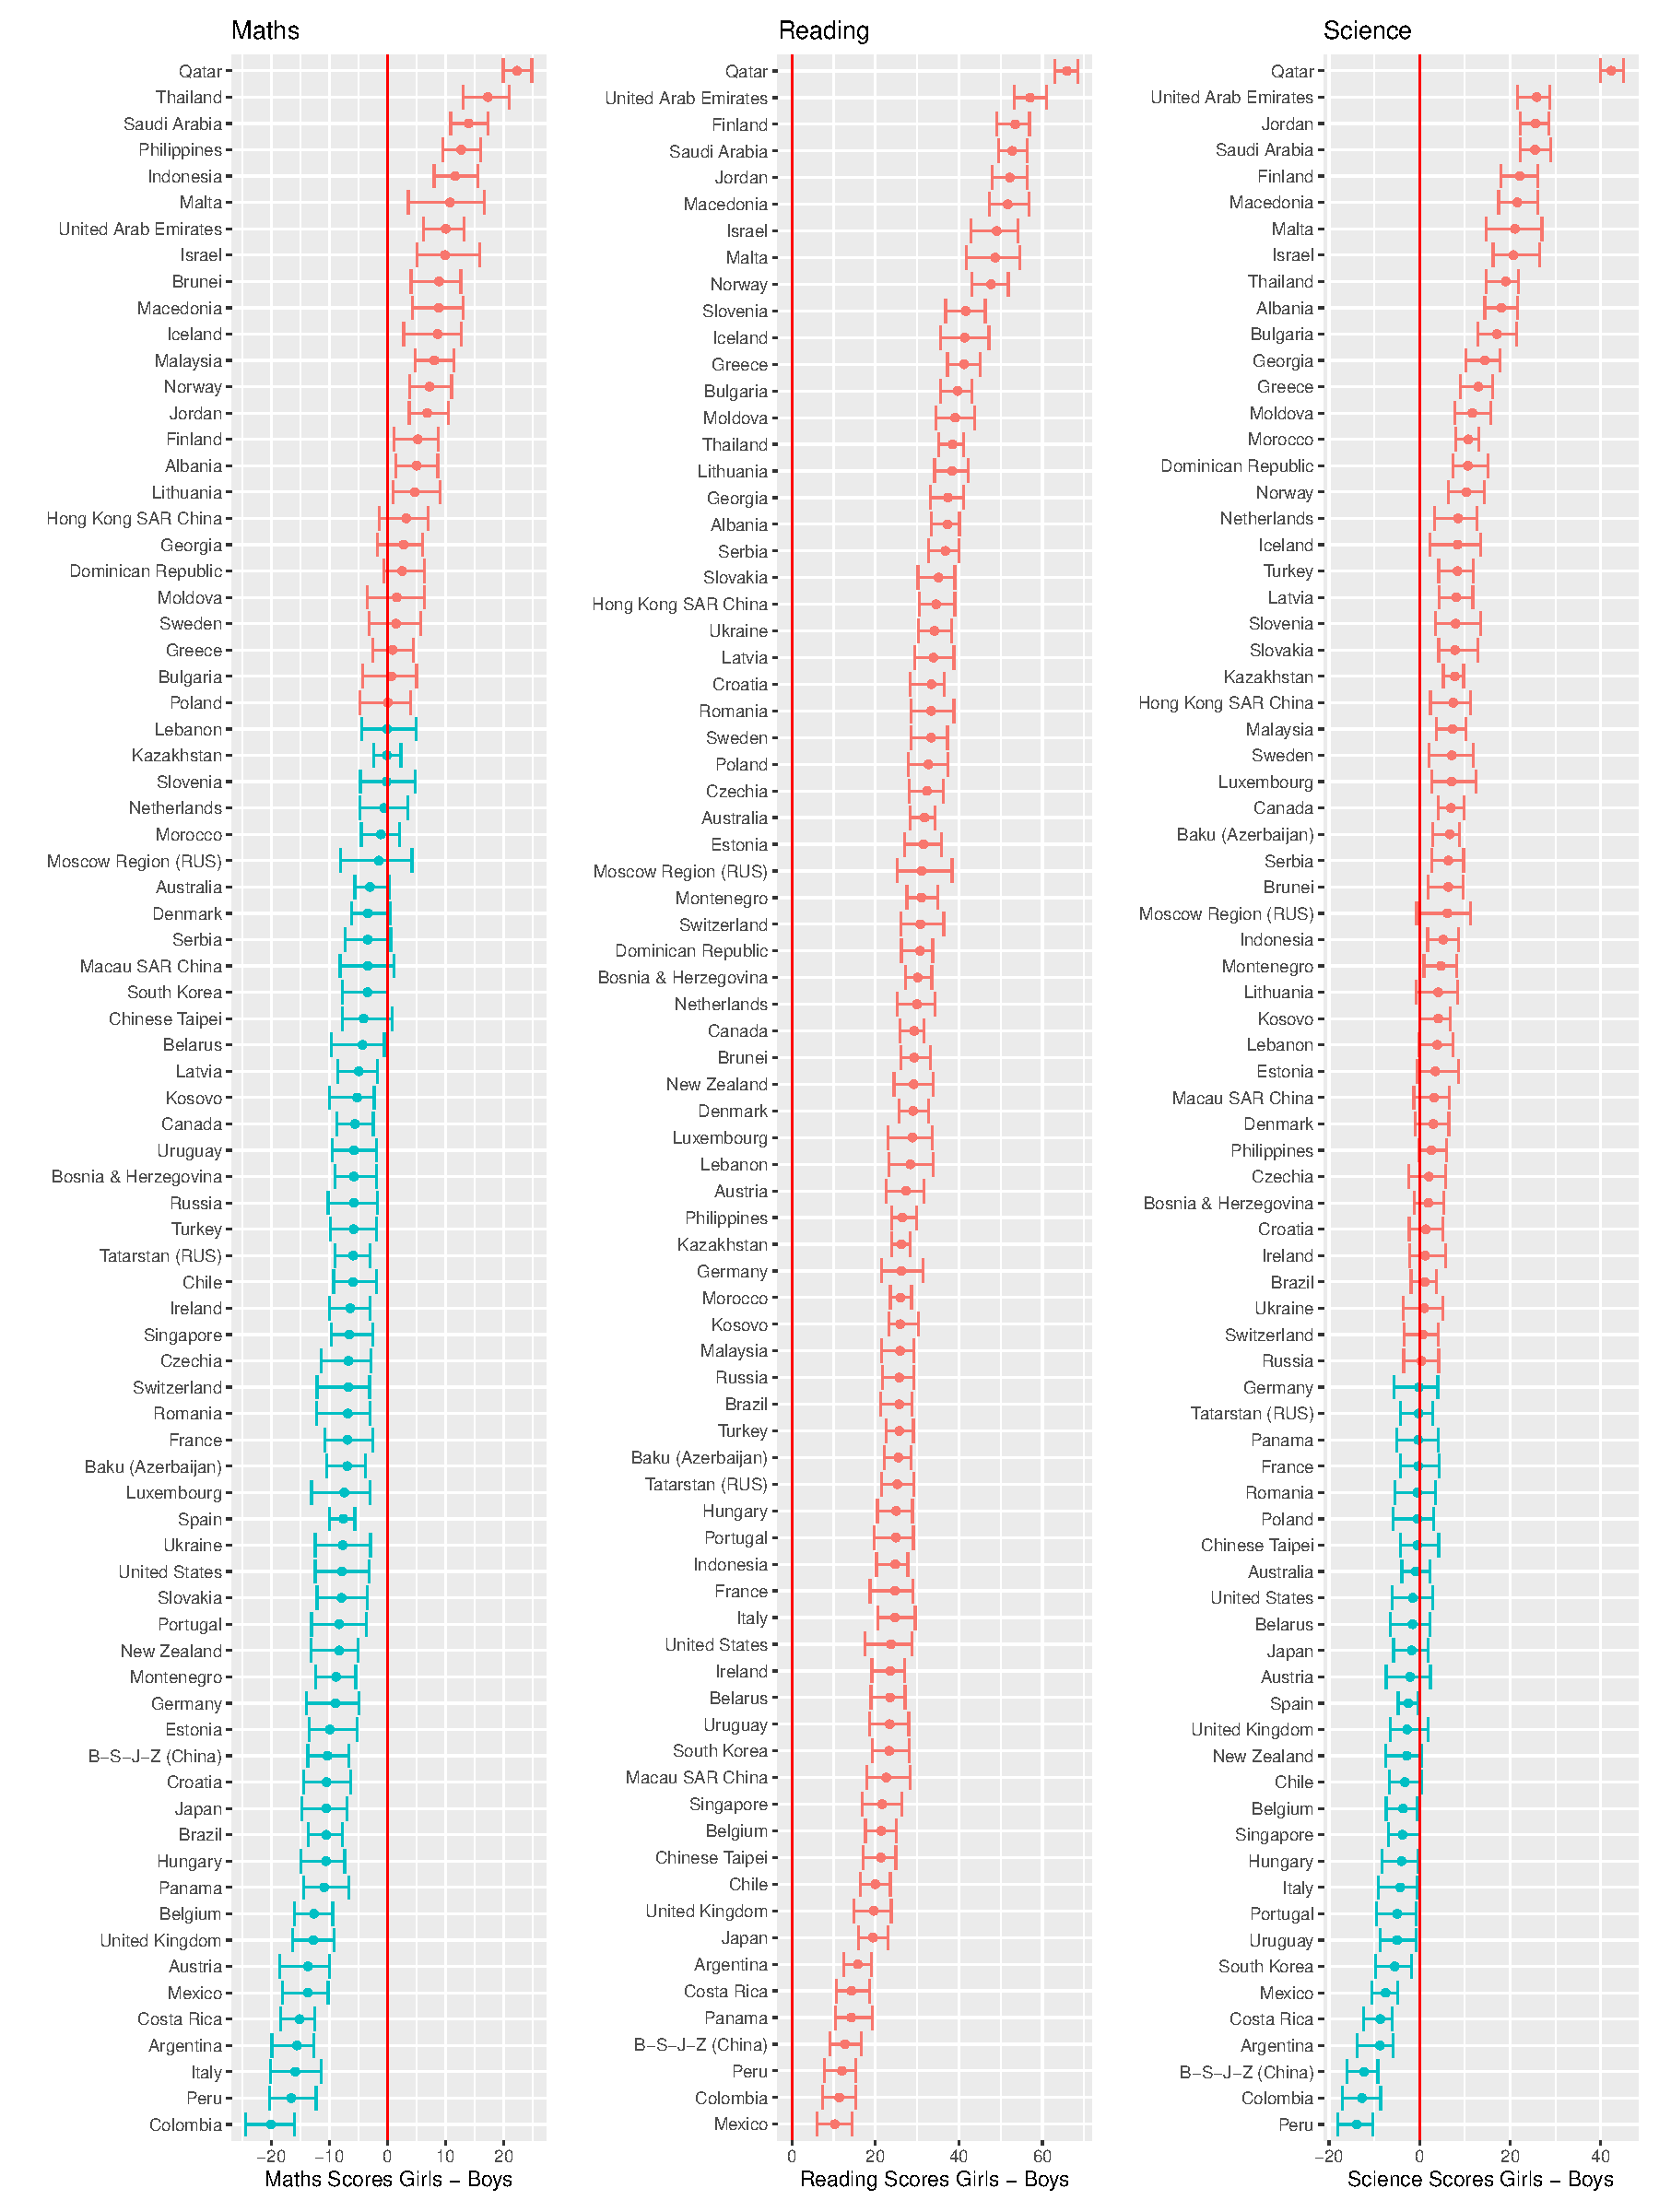
\includegraphics[width=1\linewidth]{learningtower_files/figure-latex/score-differences-1} \caption[The chart above depicts the gender gap difference in 15-year-olds' in math, reading, and science results in 2018]{The chart above depicts the gender gap difference in 15-year-olds' in math, reading, and science results in 2018. The scores to the right of the grey line represent the performances of the girls, while the scores to the left of the grey line represent the performances of the boys. One of the most intriguing conclusions we can get from this chart is that in the PISA experiment in 2018, girls from all countries outperformed boys in reading.}\label{fig:score-differences}
\end{figure}
\end{Schunk}

Figure \ref{fig:score-differences} illustrates the global disparities in
mean math, reading, and science outcomes, before we get to the plot
conclusion, let's have a look at the variables that have been plotted.
The grey line here indicates a reference point, and all of the scores to
the right of the grey line show the scores of girls in math, reading,
and science. Similarly, the scores on the left side of this grey line
indicates the scores of boys in the three disciplines. Based on figure
\ref{fig:score-differences}, because most math estimates and confidence
intervals lie to the left of the grey line, we may conclude that most
boys outperformed girls in math. In nations such as Morocco,
Netherlands, Slovenia, Kazakhstan, Poland, Bulgaria, and Greece, there
is almost no gender difference in average math scores. When we look at
the reading scores, we notice a really interesting detail which is all
girls outpaced boys in reading in all countries in 2018. The highest
reading scores were achieved by girls from Qatar, United Arab Emirates,
and Finland. Looking further into the science plot, we see an unexpected
pattern here where most countries have very little gender difference in
science scores, implying that most boys and girls perform equally well
in science. Boys from Peru, Colombia, and regions of China perform
really well in science and girls from Qatar, the United Arab Emirates,
and Jordan are the top scores for science. Figure
\ref{fig:score-differences} helps us depicts the gender gap in math,
reading, and science for all nations and regions that took part in the
2018 PISA experiment.

We gathered meaningful insights about the gender gap between girls and
boys across the world from the above figure \ref{fig:score-differences}
because this is a geographical research communication topic, the
findings will help us better comprehend the score differences in the
three educational disciplines using world maps. Let us continue to
investigate and discover patterns and correlations using map
visualisation. To illustrate the gender gap difference between girls and
boys throughout the world, we utilize the \texttt{map\_data} function to
get the latitude and longitude coordinates needed to construct a map for
our data. We connect these latitude and longitude coordinates to our
PISA data and render the world map using \texttt{geom\_polygon} function
wrapped within \CRANpkg{ggplot2} \citep{ggplot2}, the interactive
features and placement of the plots are made using \CRANpkg{plotly}
\citep{plotly} and \CRANpkg{patchwork} \citep{patchwork} packages in R.

\begin{Schunk}
\begin{figure}[H]
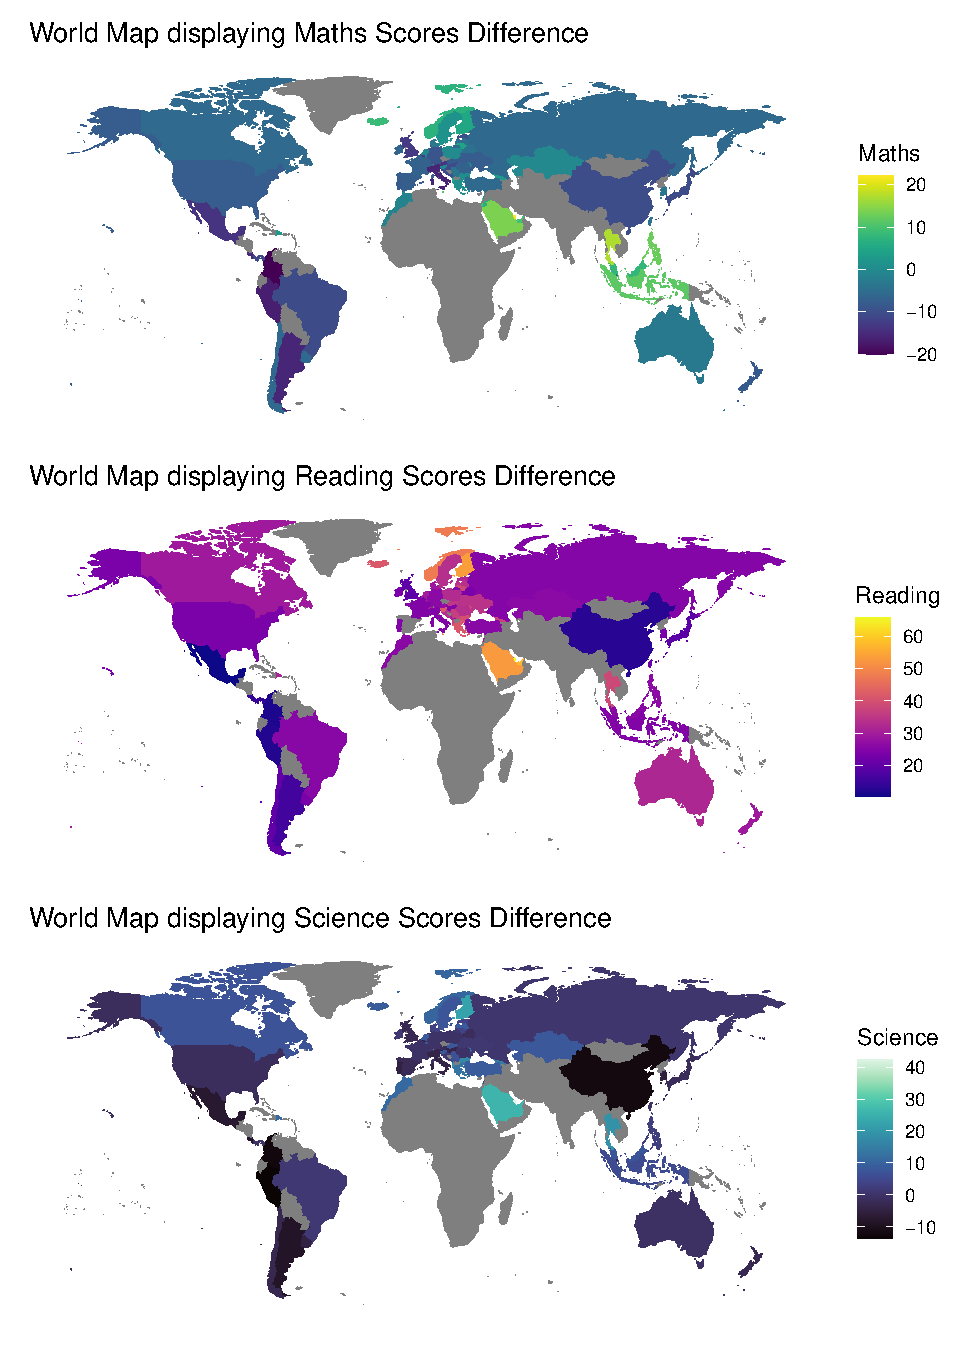
\includegraphics[width=1\linewidth]{learningtower_files/figure-latex/ggplot-maps-1} \caption[Maps showing the gender gap in math, reading, and science results between girls and boys throughout the world]{Maps showing the gender gap in math, reading, and science results between girls and boys throughout the world. The diverging colour scale makes it possible to interpret the range of scores and it also helps us intrepret the gender gap difference among these students across the globe. The legend displayed enables interpretation of the score differential for each subject across all maps. A positive score for a country indicates that girls outperformed boys in that country, whereas a negative score for a country difference indicates that boys outperformed girls in that country.The reading scores are all positive, suggesting that girls outperform boys globally in the year 2018.}\label{fig:ggplot-maps}
\end{figure}
\end{Schunk}

In the graphic \ref{fig:ggplot-maps}, we have shown the gender gap
difference between girls and boys in math, reading, and science in 2018.
Map visualization aids in the comprehension of large volumes of data in
a more efficient manner. Increases the ability to compare outcomes
across many geographies at a glance. In the illustration, we see both
positive and negative score difference scale ranges in all three maps. A
positive country score indicates that girls outperformed boys in that
country, whereas a negative country score shows that boys outscored
girls in that country. The diverging spectral color scale and the legend
of these maps makes it possible for us to deduce and identify regions
across the globe showing large gender discrepancy between girls and
boys, we can see that the most gender difference can be seen in the
reading and math scores, where most boys around the world outperform
girls in the subject of mathematics, whereas all positive reading scores
indicate that all girls around the world outperformed boys in reading in
2018. We see that there is less of a gender disparity seen in the
science scores. In addition, the color scale for scores of each subject
aids in identifying the countries that took part in the PISA experiment.
The grey colour for different geographic locations across the maps in
figure \ref{fig:ggplot-maps} indicates that these regions were not a
part of the PISA experiment in year 2018.

As a result, in this section, we have seen the gender gap scores and
striking trends between 15-year-old girls and boys in math, reading, and
science. Our main conclusion from this gender study is the performance
of girls in reading. The fewer gender disparity evident in science
scores, and the majority of boys perform better than girls in
mathematics.

\hypertarget{socioeconomic-factors}{%
\section{Socioeconomic factors}\label{socioeconomic-factors}}

Socioeconomic status is an economic and sociological complete measure of
a person's work experience, economic access to resources, and social
standing in relation to others. Do these socioeconomic factors influence
students' academic performance? In this section, we will investigate if
different socioeconomic factors owned by a family have a significant
impact on a student's academic performance. The student dataset in the
\CRANpkg{learningtower} package comprises scores of 15-year-olds from
triennial testing across the world. This dataset also includes
information about their parents' education, family wealth, gender, and
ownership of computers, internet, cars, books, rooms, desks, and
dishwashers. In this section, we will mainly explore intriguing figures
and derive some fascinating aspects of the influence of a few
socioeconomic factors on student performance in math, reading, and
science. Before we go on to our socioeconomic determinants and their
impact on students, figure \ref{fig:corr-plot} shows how the math,
reading, and science scores are strongly positively correlated to one
another.

\begin{Schunk}
\begin{figure}[H]
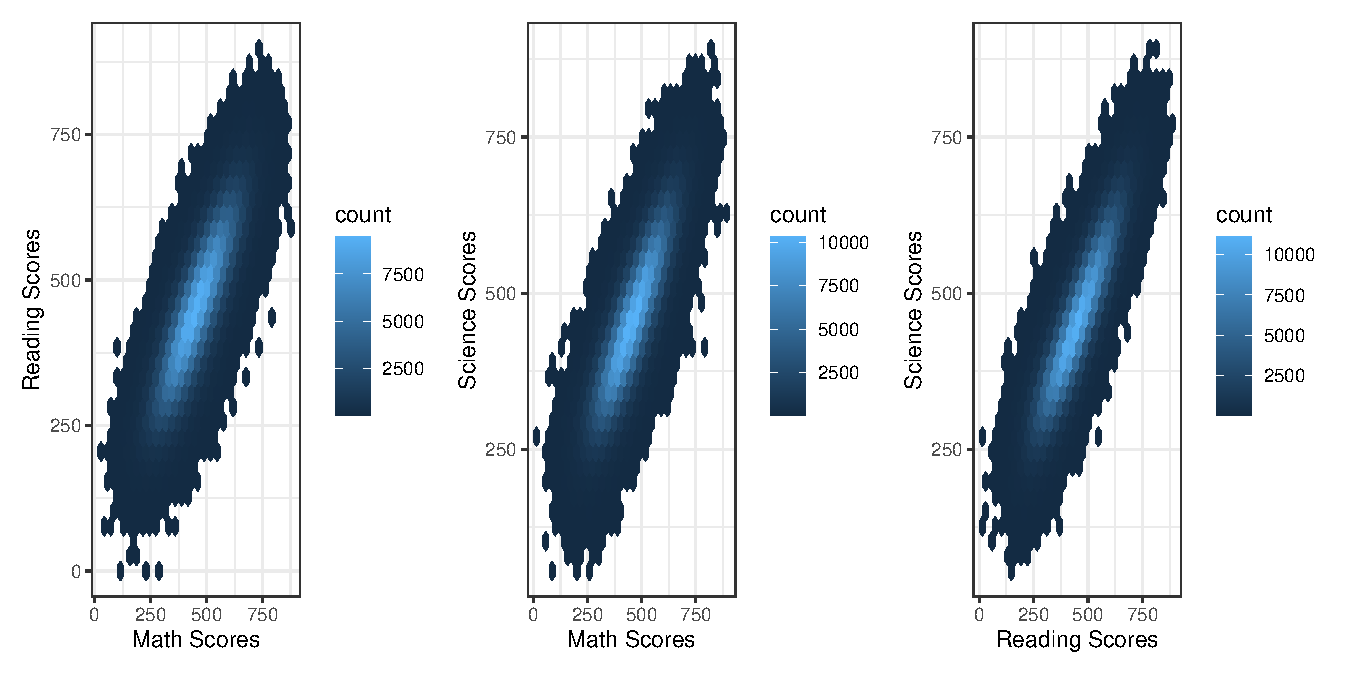
\includegraphics[width=1\linewidth]{learningtower_files/figure-latex/corr-plot-1} \caption[The scatterplot displays the relationship between math, reading, and science scores for all PISA countries that participated in the experiment in 2018]{The scatterplot displays the relationship between math, reading, and science scores for all PISA countries that participated in the experiment in 2018. This scatterplot shows that all three subjects have a significant and positive correlation with one another.}\label{fig:corr-plot}
\end{figure}
\end{Schunk}

We plotted all three scores against each other using the
\texttt{geom\_hex()} function available under the \CRANpkg{ggplot2}
\citep{ggplot2} package in R. The figure \ref{fig:corr-plot} help us us
reveal the relationship between these three subjects allowing us to
deduce that math, science, and reading scores are positively and
significantly correlated with one another, implying that when we inspect
and analyse the many socioeconomic determinants, we would get comparable
outcomes with each subject math, reading or science along with the
influence of desired socioeconomic factor. As a result of seeing this
substantially positive association between all three subjects for all
the countries that participated in the PISA experiment in 2018, the
developers decided to show the effect of socioeconomic variables on
average math scores only due to highly positive correlation since the
other two subjects will show similar patterns as well. Let us further
explore the impact of a few socioeconomic factors on the students'
score.

Parents qualification is and will always be a vital element of childhood
development. As previously stated, the student dataset in the package
includes information regarding the parents qualification. In this
section, we will investigate if both the mother's and father's
qualifications have a significant impact on the child's performance. The
mother's education and father's education variables are originally
recorded in the student dataset in the \CRANpkg{learningtower} package
at distinct levels which are less than ISCED1 equivalent to ISCED 0,
ISCED 1, ISCED 2, ISCED 3A and ISCED 3B, C. The International Standard
Classification of Education, (ISCED) decides and classifies these
levels, where level 0 indicates pre-primary education or no education at
all, level 1 indicates primary education or the first stage of basic
education, level 2 indicates lower secondary education or the second
stage of basic education, and level 3 indicates upper secondary
education. ISCED level 3 have been further classified into three
distinct levels, with ideally very little difference in their
classification. This may also be found in the publication
\href{https://www.oecd.org/education/1841854.pdf}{Classifying
Educational Programmes} \citep{isced} published by ISCED. To determine
the impact of parents qualification we first create \texttt{data.frames}
that are categorized by the various countries and regions and grouped by
the father's and mother's qualification. We next compute the weighted
mean average of math scores while accounting for student weights.
Furthermore, we re-factored the parents qualification variable based on
the multiple levels of classification, dividing it into four unique
levels of education, namely early childhood, primary, lower, and
secondary education. Furthermore, we display the weighted math average
versus qualification colored by the re factored qualifications levels
for both the mother and father using the \texttt{geom\_quasirandom}
function wrapped within \CRANpkg{ggplot2} \citep{ggplot2}, we further
plot this with the help of \CRANpkg{viridis} \citep{viridis} and
\CRANpkg{patchwork} \citep{patchwork} packages in R.

\begin{Schunk}
\begin{figure}[H]
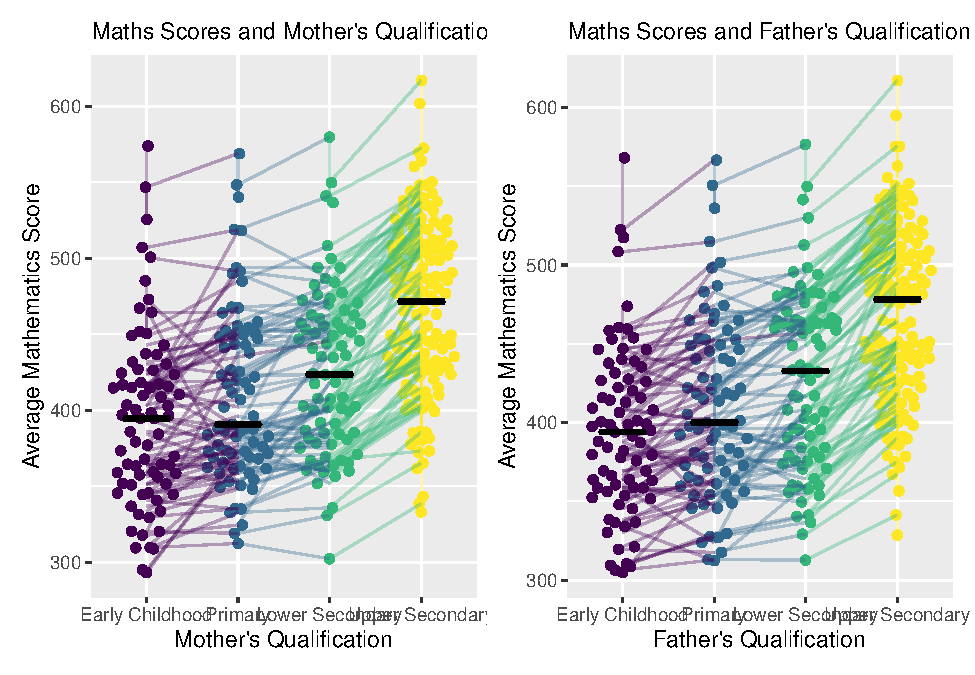
\includegraphics[width=1\linewidth]{learningtower_files/figure-latex/qual-plot-1} \caption[The impact of parents' education on their children's academic progress is depicted in this graph]{The impact of parents' education on their children's academic progress is depicted in this graph. When the parents have greater levels of education, we see a considerable rise in scores and an increase in the median of scores for each category, as shown in the figure. In comparison to parents with lower levels of education qualifications. Parents who have tend to have upper secondary qualification or equivalent credentials their children are more likely to perform better in academics when compared with parent having lesser levels of qualifications.}\label{fig:qual-plot}
\end{figure}
\end{Schunk}

The figure \ref{fig:qual-plot} depicts the impact of mothers' and
fathers' qualifications on students academic performance. The figure
\ref{fig:qual-plot} allows us to deduce a very important and remarkable
insight in which we see a constant increase in the students' academic
performance when both mother and father qualifications shift towards
higher levels of education. The bold horizontal black lines that we see
in each category for mother's and father's qualification here represent
the category's median score. As the parent attains higher
qualifications, we notice an increasing trend in these medians for each
category. Taking a closer look at the figure \ref{fig:qual-plot}, we can
see that there is a considerable boost in scores when both the mother
and father have upper secondary education. Furthermore, utilizing
\texttt{geom\_quasirandom()} function available in the
\CRANpkg{ggbeeswarm} \citep{ggbeeswarm} ggbeeswarm makes this plot more
accessible and understandable by providing a way to offset points inside
categories to prevent overplotting. Thus, we can clearly see that both
the mother's and father's qualifications have a significant influence on
the student's academic performance, with the more educated the parent,
the more likely their offspring are to perform well academically.

Television is one of humanity's greatest inventions; it is one of the
assets that has had a significant impact and influence on humans. In
this segment of the article, we investigate the influence of television
in many countries, as well as whether this technology has a significant
impact on students' academic performance. The television variables that
are recorded in the student dataset is a factor variable that records
whether or not the students participating in this study have a
television and, if they do, the quantity of televisions per family is
recorded via the PISA survey. Furthermore, because we are interested in
researching the impact of these television on the students' scores, the
television variable initially recorded has four levels: No TV, 1 TV, 2
TVs, or 3+TVs. We are also interested in visualising the confidence
intervals for each of these levels in order to determine the uncertainty
of the results at each level. We begin with initially creating a
\texttt{data.frame} that is grouped by country and the number of
television per household for each country. Next we fit a linear model to
the math average and distinct television categories for each country in
the 2018 PISA data and finally plot the television impact for all
countries sorted as per the slope with the help of the functions
available in the \CRANpkg{ggplot2} \citep{ggplot2} package.

\begin{Schunk}
\begin{figure}[H]
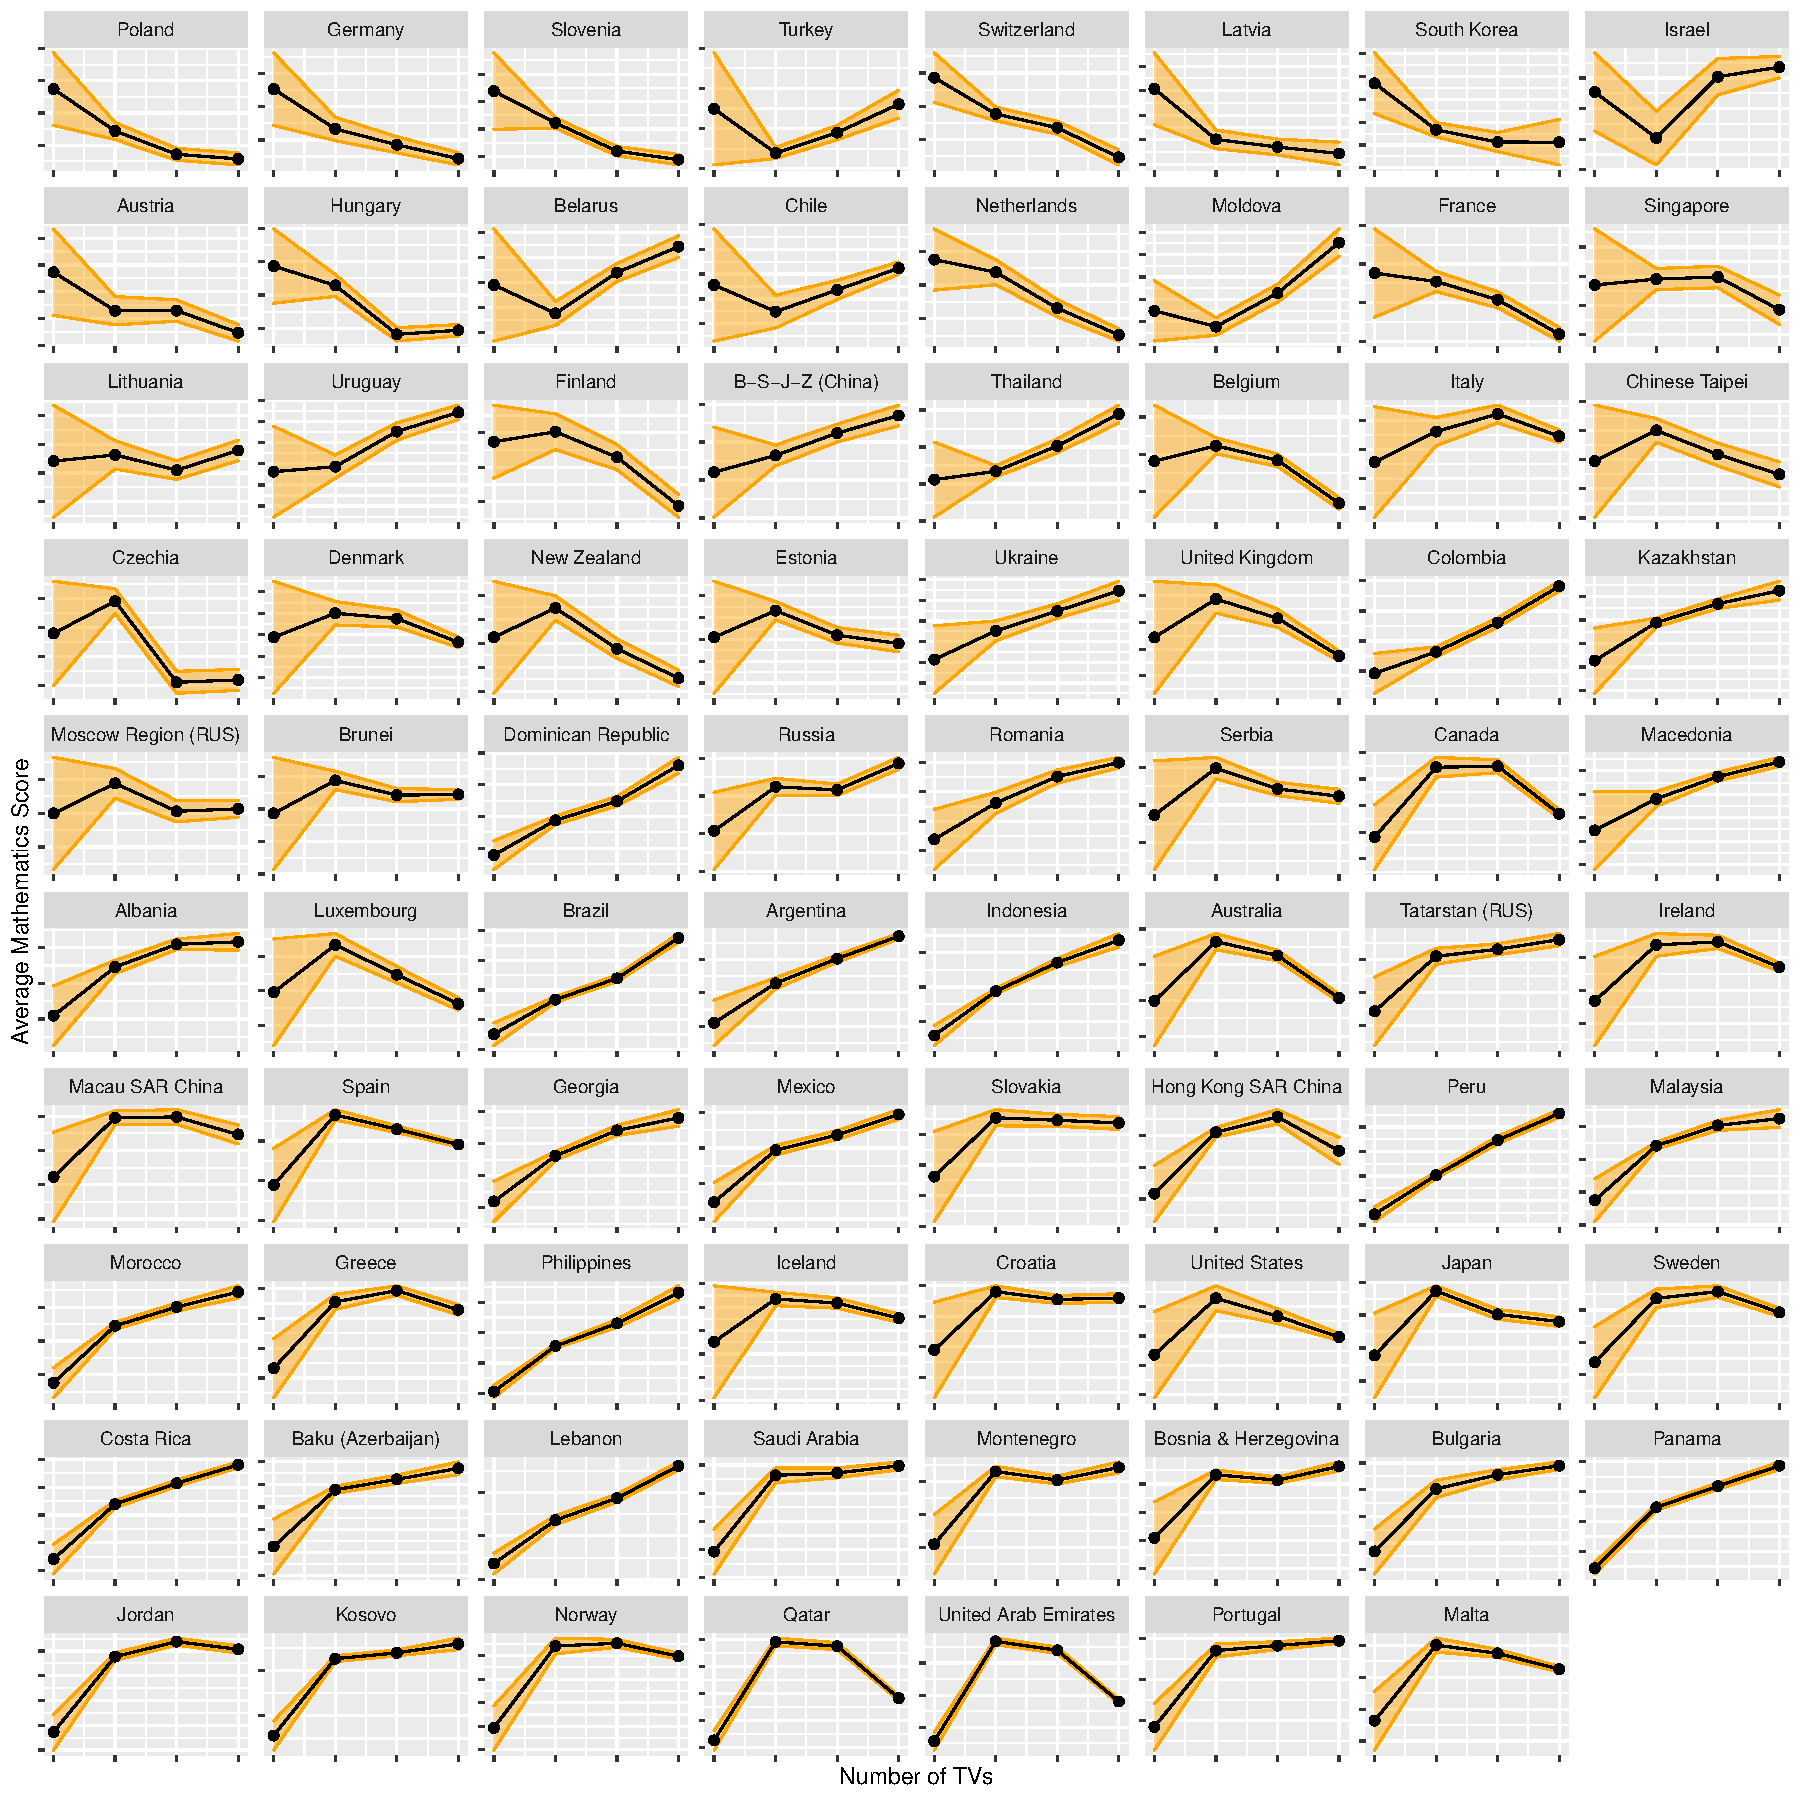
\includegraphics[width=1\linewidth]{learningtower_files/figure-latex/tv-plot-1} \caption[Relationship  between number of TVs in a household and average math scores across countries]{Relationship  between number of TVs in a household and average math scores across countries. Number of TVs ranges from 0 to 3 or more. The orange bands indicate 95 percent standard confidence intervals. The impact of television on student performance is a contentious issue. It is interesting that in some countries for example in Malta and Portugalthe effect appears to be positive, but in other countries like Poland and Germany there is a decline in average math scores.}\label{fig:tv-plot}
\end{figure}
\end{Schunk}

In the figure \ref{fig:tv-plot}, we can see highly striking patterns as
well as a significant influence of television on students' academic
performance. We have arranged the nations in the figure
\ref{fig:tv-plot} according to the slope of math average scores fitted
against the different levels of television described previously. Poland,
Germany, Slovenia, and Turkey have a lower influence of television on
student performance, whereas Malta, Portugal, United Arab Emirates and
Qatar have a rising tendency and therefore a larger impact of television
on students' performance. Furthermore, the confidence interval plotted
in the figure \ref{fig:tv-plot} show that there is a lot of uncertainty
in the level of scores when a household does not possess a TV in the
majority of the countries. Taking a closer look at the figure
\ref{fig:tv-plot} we observe that when the slope of television increases
in countries, the confidence interval of such countries becomes
narrower. Hence depending on your wealth and where you live, television
can be a valuable asset since it has a notable effect on a student's
academic performance.

We've always heard and read that books play an important role in early
childhood because they assist learners develop emotional intelligence
and creativity. However, the developers of \CRANpkg{learningtower}
package intended to invest if books, has a significant influence on the
students score. The book variable is initially recorded in the student
dataset has been categorized in the following levels 0-10, 11-25,
26-100, 101-200, and more than 500 books. We will do a similar
investigation as we did when we investigated the effect of television.
First, we construct a \texttt{data.frame} that is grouped by the
different levels of books and countries. In addition, we calculated the
confidence interval using the method to account for the uncertainty
associated with the scores for the different categories of books. We
subsequently fit a linear model with the average math score and each
level of book categories to derive a coefficient or slope for each
country. Finally, plot the country and score estimations for each
country, ordered according to slope with help of the functions available
in the \CRANpkg{ggplot2} \citep{ggplot2} package.

\begin{Schunk}
\begin{figure}[H]
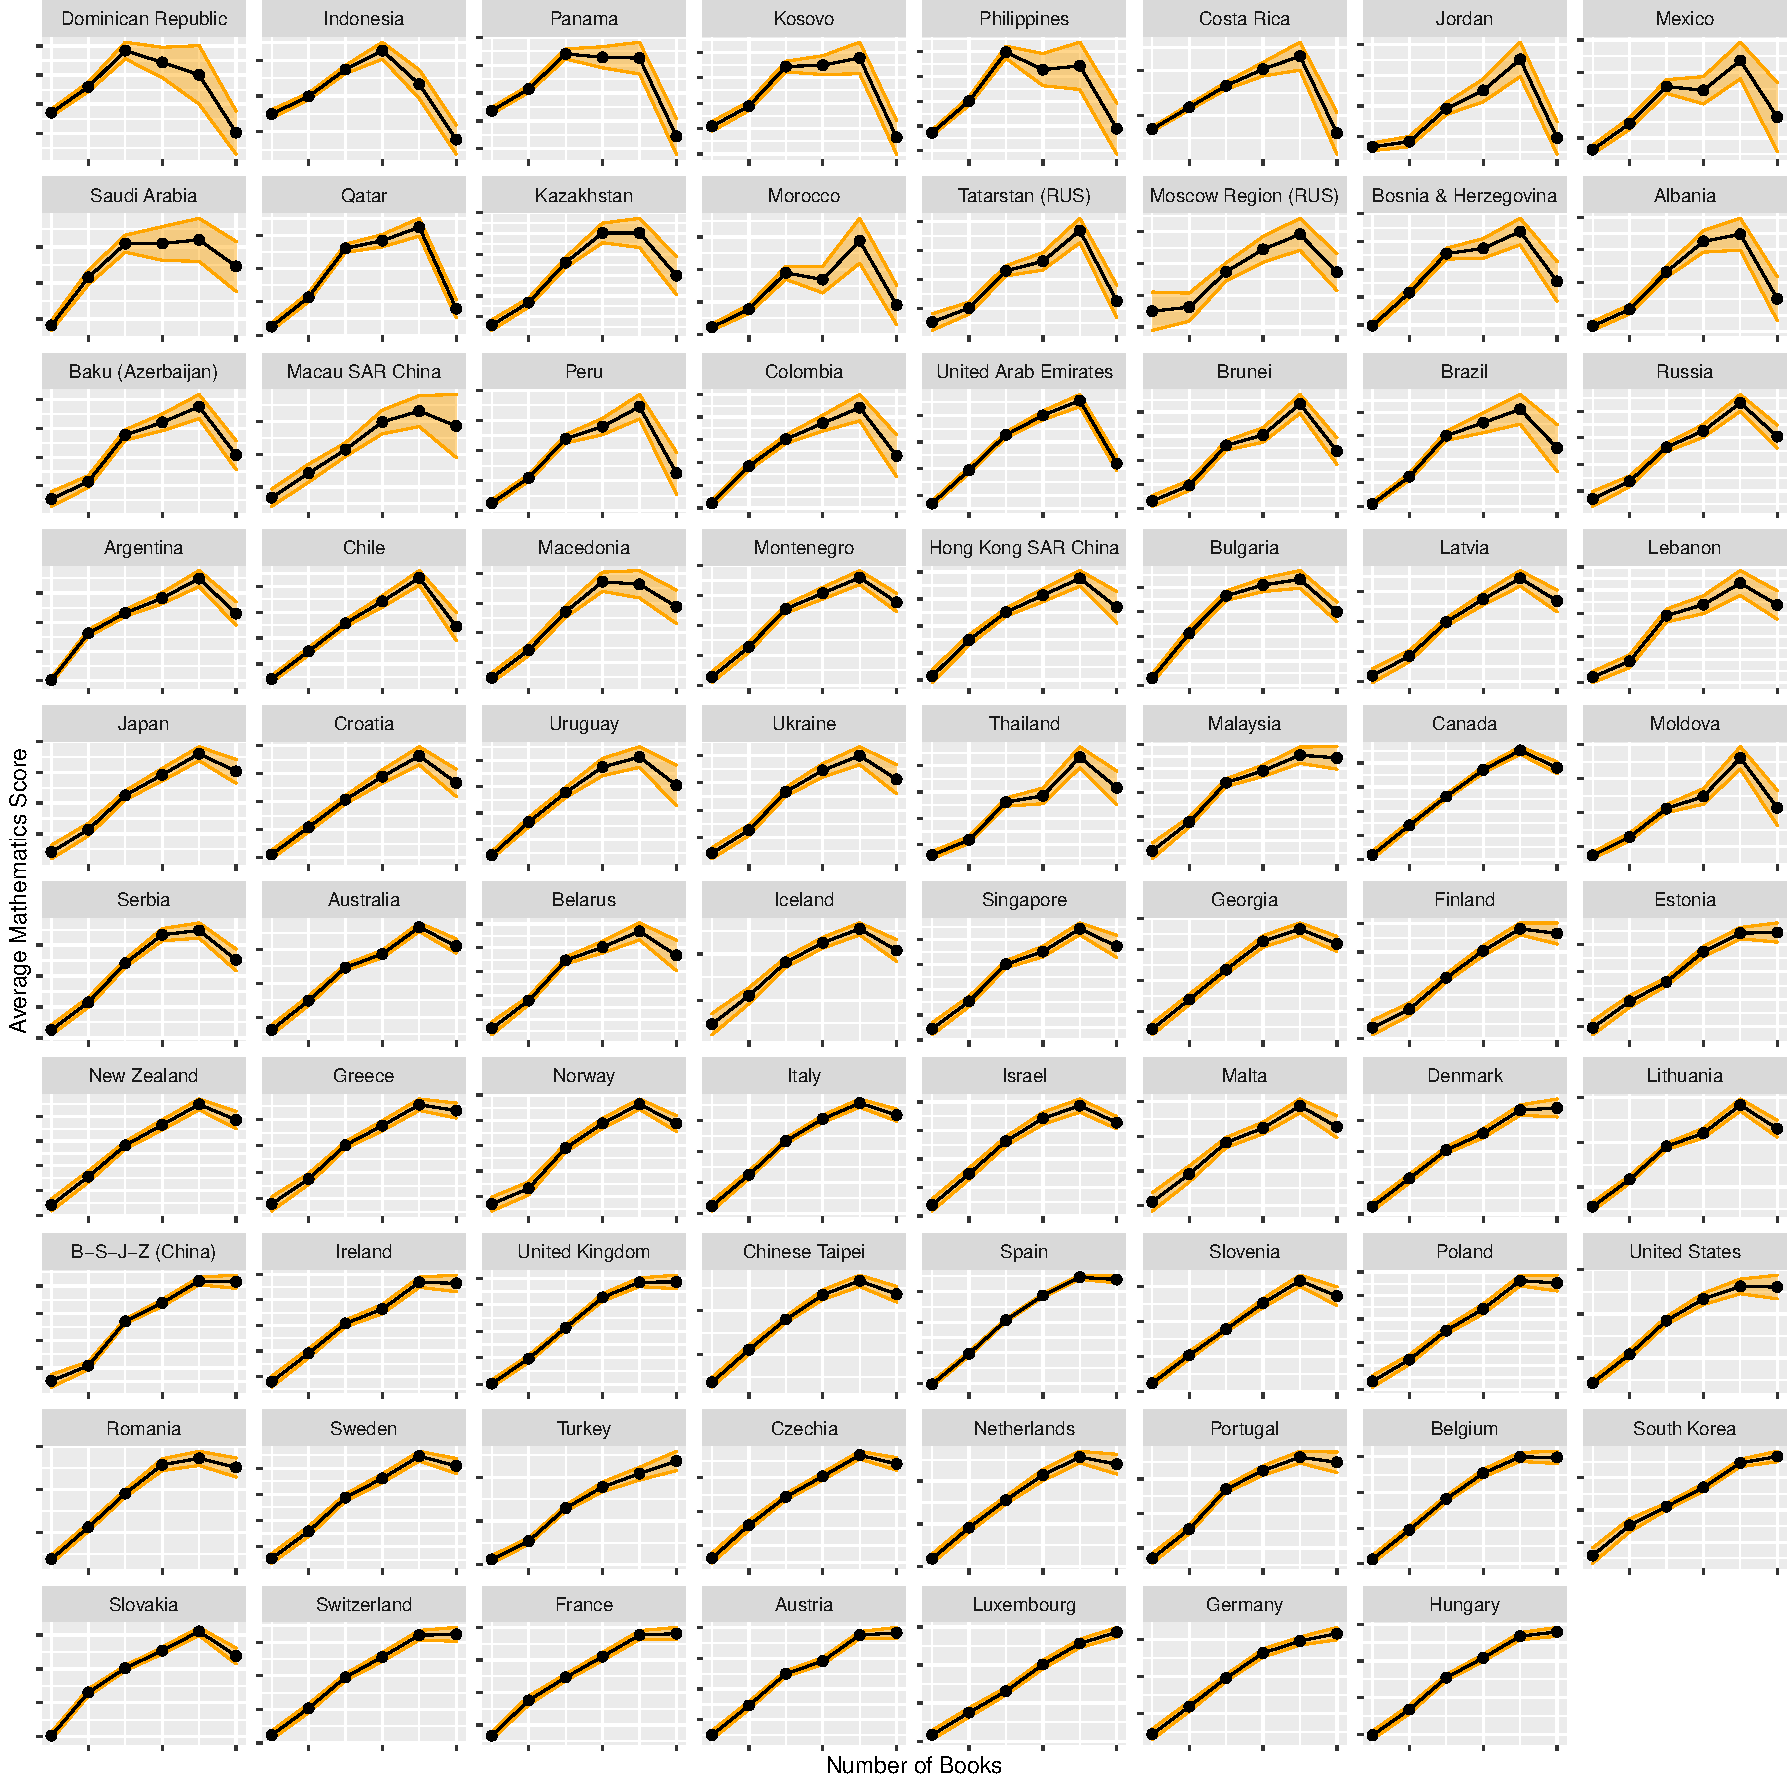
\includegraphics[width=1\linewidth]{learningtower_files/figure-latex/book-plot-1} \caption[Impact of the number of books on average math score]{Impact of the number of books on average math score. Number of books ranges from 0 to 500 and more. 95 percent standard confidence bands shown in orange. Math scores generally increase as the number of books increases. Averages for some countries at the higher number of books are less reliable, and hence the decline reflects more that there are few households with this many books than a true decline.}\label{fig:book-plot}
\end{figure}
\end{Schunk}

In the figure \ref{fig:book-plot}, we can see the different countries
arranged by slope and their correlation with math score estimation for
each of the book categories. Taking a detailed look at the figure
\ref{fig:book-plot}, we deduced that the more books a family possesses,
the more likely it is that its children will perform well academically.
Looking at the graph, we can notice a rising tendency as the quantity of
books per household increases. Furthermore, we see a decline in the
score when the category contains more than 500 books, owing to the lack
of data in such categories. Because ideally there are extremely few
households that own more than 500 books. In this scenario, we also
examine the confidence intervals of our plots to better understand the
lower and upper bounds of the math score estimation. The confidence
intervals in each of the categories are not particularly very broad
except for a few countries like Dominican Republic, Philippines and
Saudi Arabia. In addition, arranging the graph by slope allows us to
understand the impact of books in different countries. Despite the fact
that most countries have a significant influence on books per household,
we can see in this graph that most countries have a significant impact
on books per household. We may state that the Dominican Republic,
Indonesia, and Panama have witnesses a slightly lower impact of owing
books than the countries of Luxembourg, Germany, and Hungary. As a
result, we may conclude that having a greater quantity of books in a
home will undoubtedly benefit a student's academic performance.

Students are becoming autonomous, adept members and researchers as they
advance in technology and usage of computers and the internet. However,
let us investigate if having a computer with internet access at the age
of 15 has a positive or negative impact on student academic achievement.
We will plot the average math results of the several nations that
participated in the PISA experiment in 2018 to determine the effect of
owning a computer and having access to the internet. This necessitates
the creation of a \texttt{data.frame} that is grouped by the nations and
the frequency of or whether the student possesses a computer or not, as
well as a students' access to the internet or not. We will plot this
result against the weighted average mathematical score to determine the
influence of various of television and internet on the student academic
performance using the several functions available in the
\CRANpkg{ggplot2} \citep{ggplot2} package.

\begin{Schunk}
\begin{figure}[H]
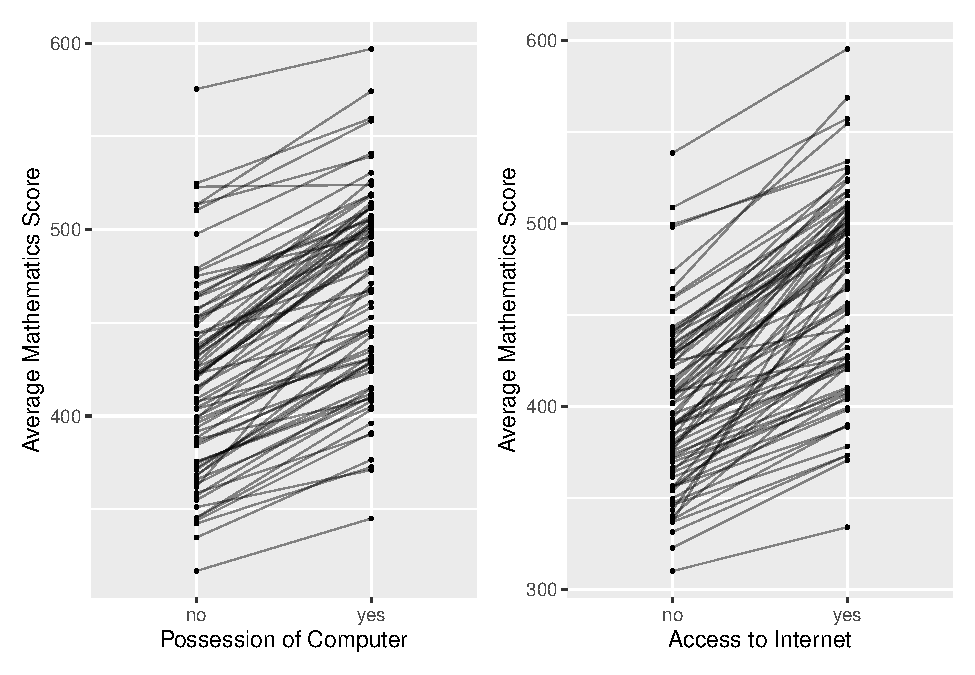
\includegraphics[width=1\linewidth]{learningtower_files/figure-latex/compint-plot-1} \caption[Computers and the Internet are two of the most important inventions in the history of technology]{Computers and the Internet are two of the most important inventions in the history of technology. In this figure, we observe the impact of owning a computer and having access to the internet on 15-year-old students all over the world. A remarkable finding from the plot is that all nations have higher scores in student performance when they own a computer and have access to the internet.}\label{fig:compint-plot}
\end{figure}
\end{Schunk}

In the figure \ref{fig:compint-plot}, we see some absolutely fascinating
and astonishing insights that might help education policymakers make
decisions. This data allows us to conclude that students who own a
computer and have access to the internet consistently outperform
students who do not own a computer or have access to the internet at
all. Interestingly, we regard these as actionable information for all
countries participating in the PISA study in 2018. No country has
exempted from this findings. Thus, a 15-year-old student's access to a
computer and the internet is unquestionably has significant positive
influence on their academic performance.

\hypertarget{temporal-trend}{%
\section{Temporal trend}\label{temporal-trend}}

In this section of analysis, we look at the temporal trends noticed in
Australia. The release of PISA results in 2018 led to several headlines
on the decline in scores recorded in Australia. In this section, we will
determine whether this decrease is indeed significant or whether there
are any other aspects to consider when comparing country rankings. To
better comprehend Australia's scores and trends since 2000, the
developers of the \CRANpkg{learningtower} package, feel it is
appropriate to illustrate the temporal trend of Australia in comparison
to a few other nations. We evaluate these countries performance using a
statistical procedure bootstrapping using the \texttt{map\_dfr} function
which re-samples a single dataset to generate a large number of
simulated samples. We will compare the results of these bootstrap
samples across all the years they participated in PISA and highlight a
few countries with help of \CRANpkg{gghighlight} \citep{gghighlight}
performance to compare with Australia's

\begin{Schunk}
\begin{figure}[H]
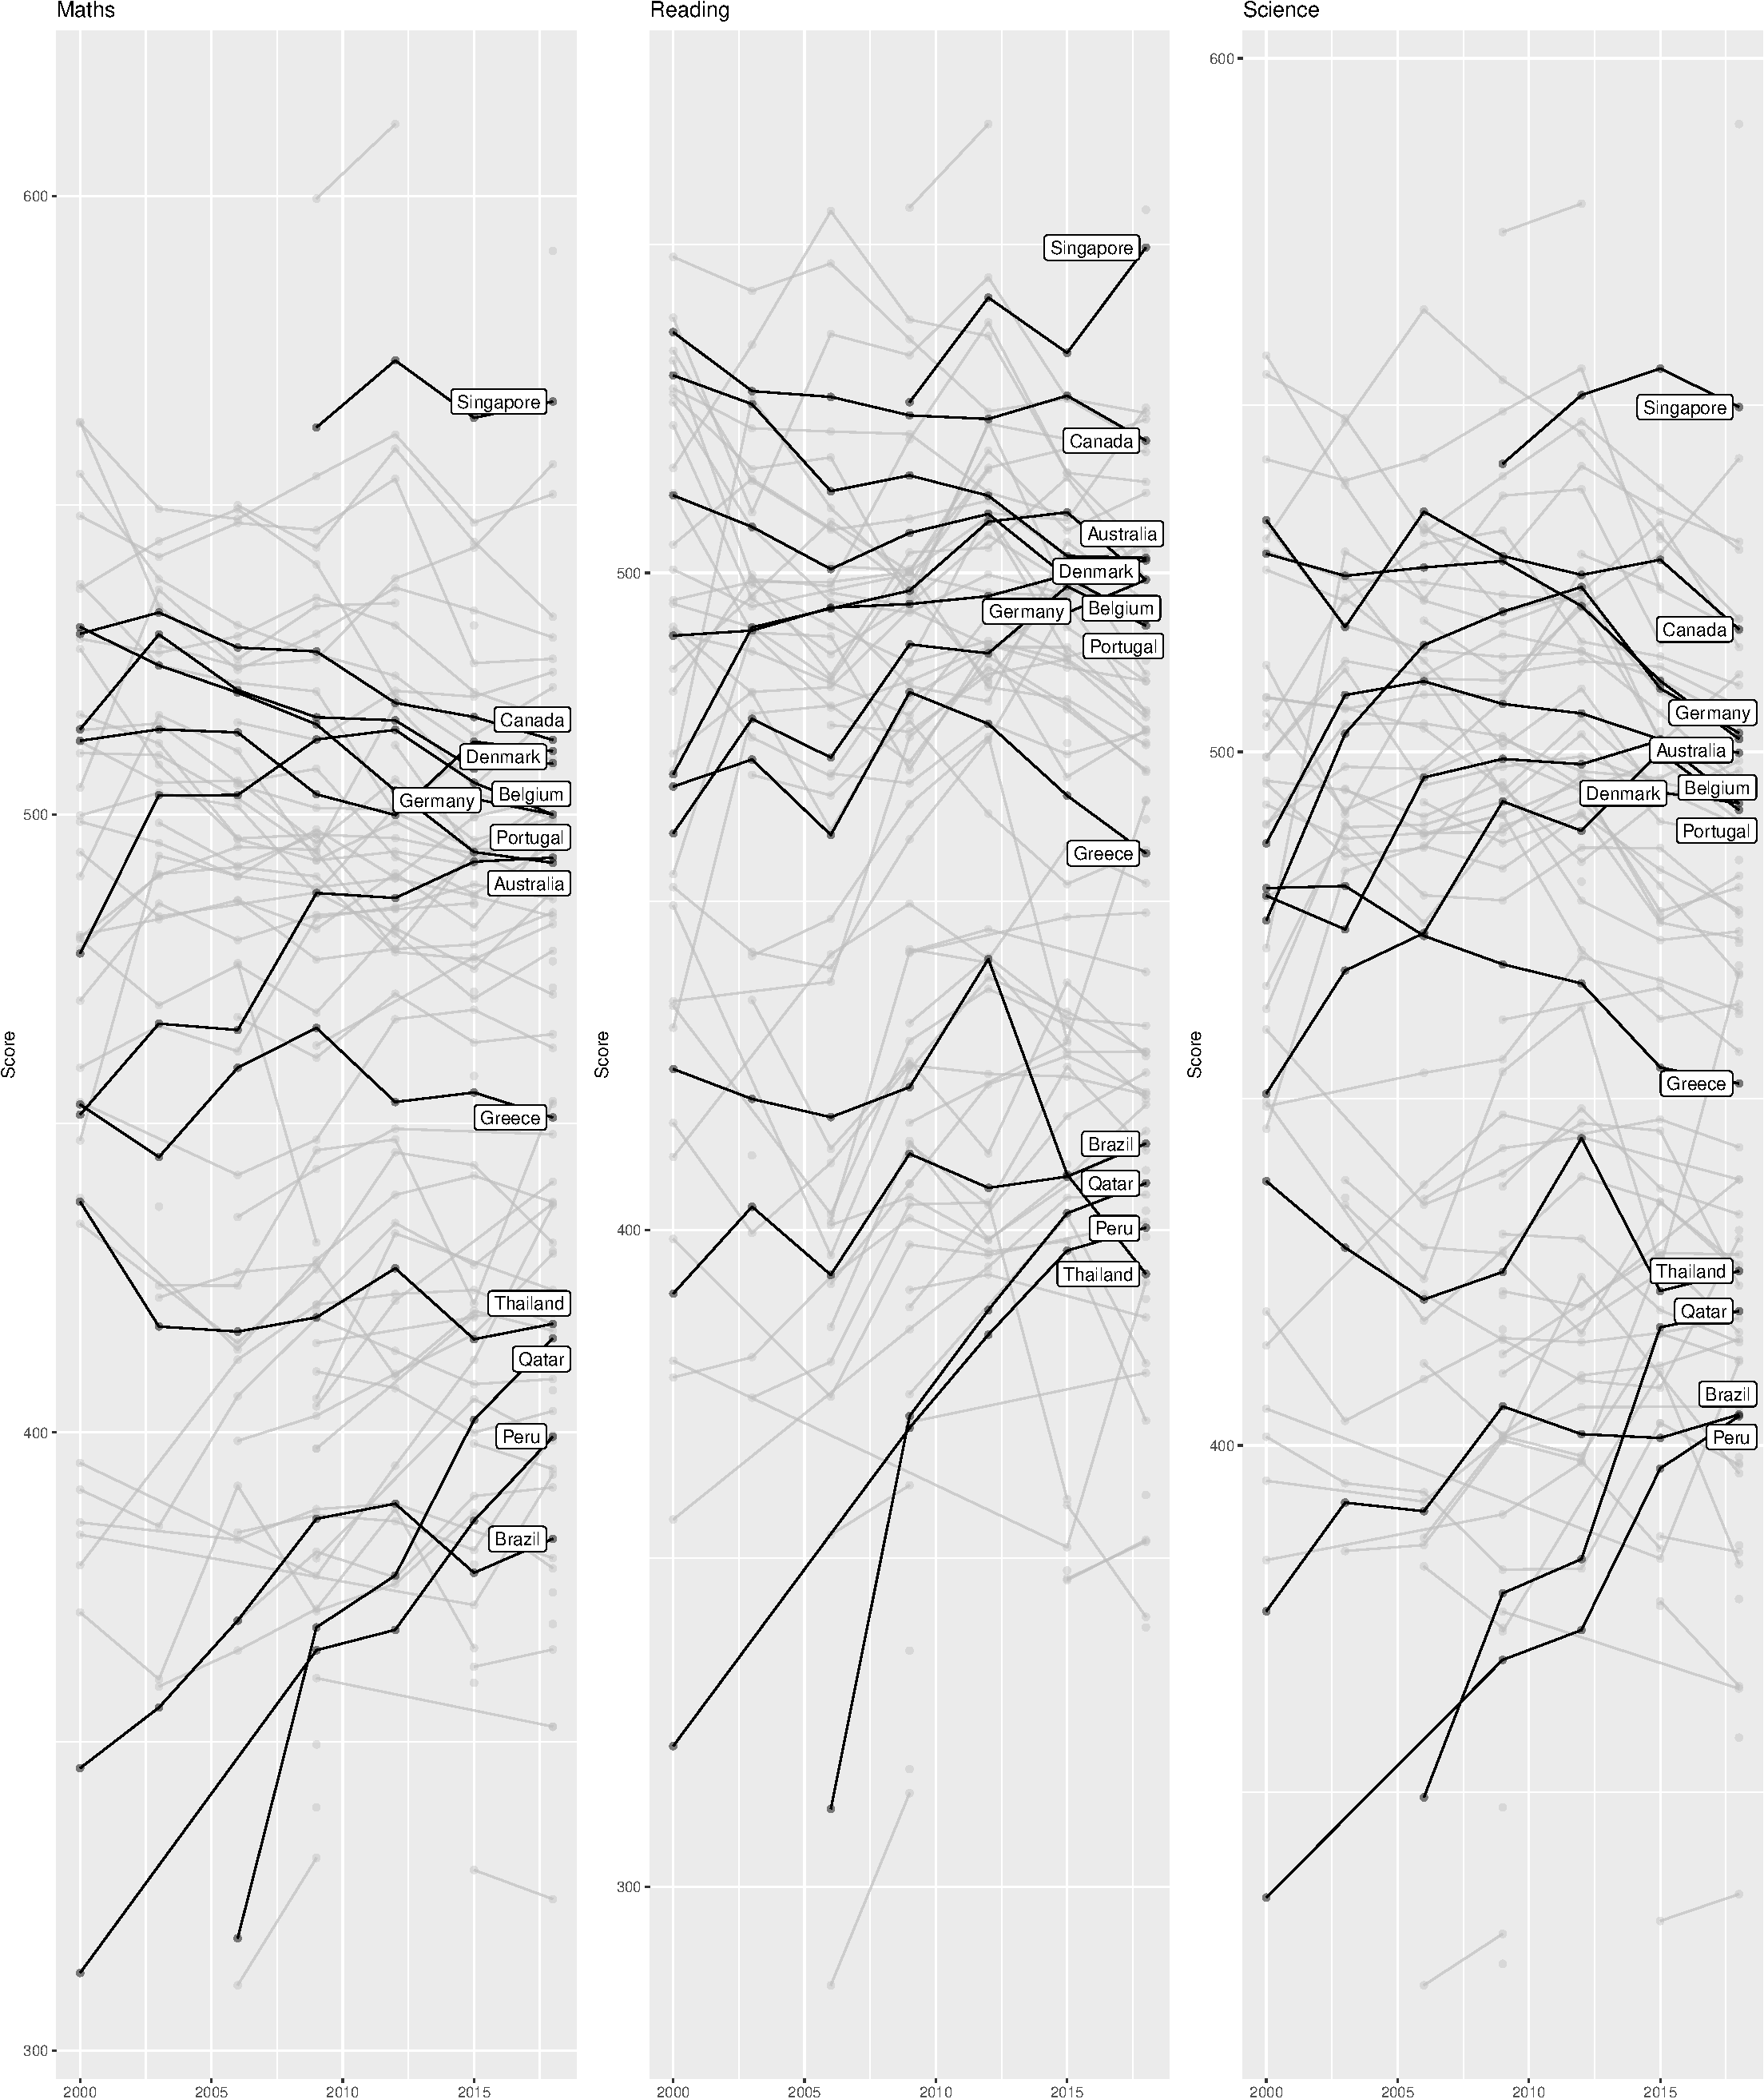
\includegraphics[width=1\linewidth]{learningtower_files/figure-latex/bs-plot-1} \caption[Temporal patterns in math, reading, and science in a variety of countries]{Temporal patterns in math, reading, and science in a variety of countries. The highlighted countries in the chart help us infer Australia's performance in contrast to the other countries; we can see that Australia's scores have always been among the highest in the PISA survey throughout all years.}\label{fig:bs-plot}
\end{figure}
\end{Schunk}

Taking a deeper look at the figure \ref{fig:bs-plot} and comparing the
Australia scores to a few of the selected countries, we notice the
changing scales of their scores in all three plots of math, reading, and
science and we infer that Australia's performance has been is much
better than than majority of the countries. To deepen our understanding
of the topic, we compare Indonesia's, Qatar's or Peru's results to those
of Australia and observe and increasing pattern for all of them but
Australia. On closer examination we witness that the highest score for
Indonesia, Qatar or Peru are initially low scores and this increases
further. However, Australia's performance in the PISA was initially a
top achievement, and it has only drops by a few points. Though the
temporal trend of Australia displays a declining tendency, this is due
to the fact that Australia initially performed very well in the PISA
experiment and has only decreased it scores by a few points each year,
remaining in one of the top scores of the PISA research until the year
2018. As a result, we infer that Australian's performance has declined
over time but the country has remained on the list of top scores
countries for all of the years this PISA research has been done. Using a
similar notion, we conclude that countries with lower initial PISA
results have a tendency to increase their score each time the PISA exam
is taken whilst countries that have previously established a standard
with great score results like Australia may witness a decreasing trend
in the scores but optimally the scores has decrease by a few points only
thus not making the the declining trend a significant measure of
performance. In addition, to understand this better, we have a animation
plotted using \CRANpkg{gganimate} \citep{gganimate} the that explains
how performance can only be compared among scales and not based on
scores or any other characteristics with respect to several other
countries that participated in the PISA experiment.

\begin{Schunk}
\begin{figure}
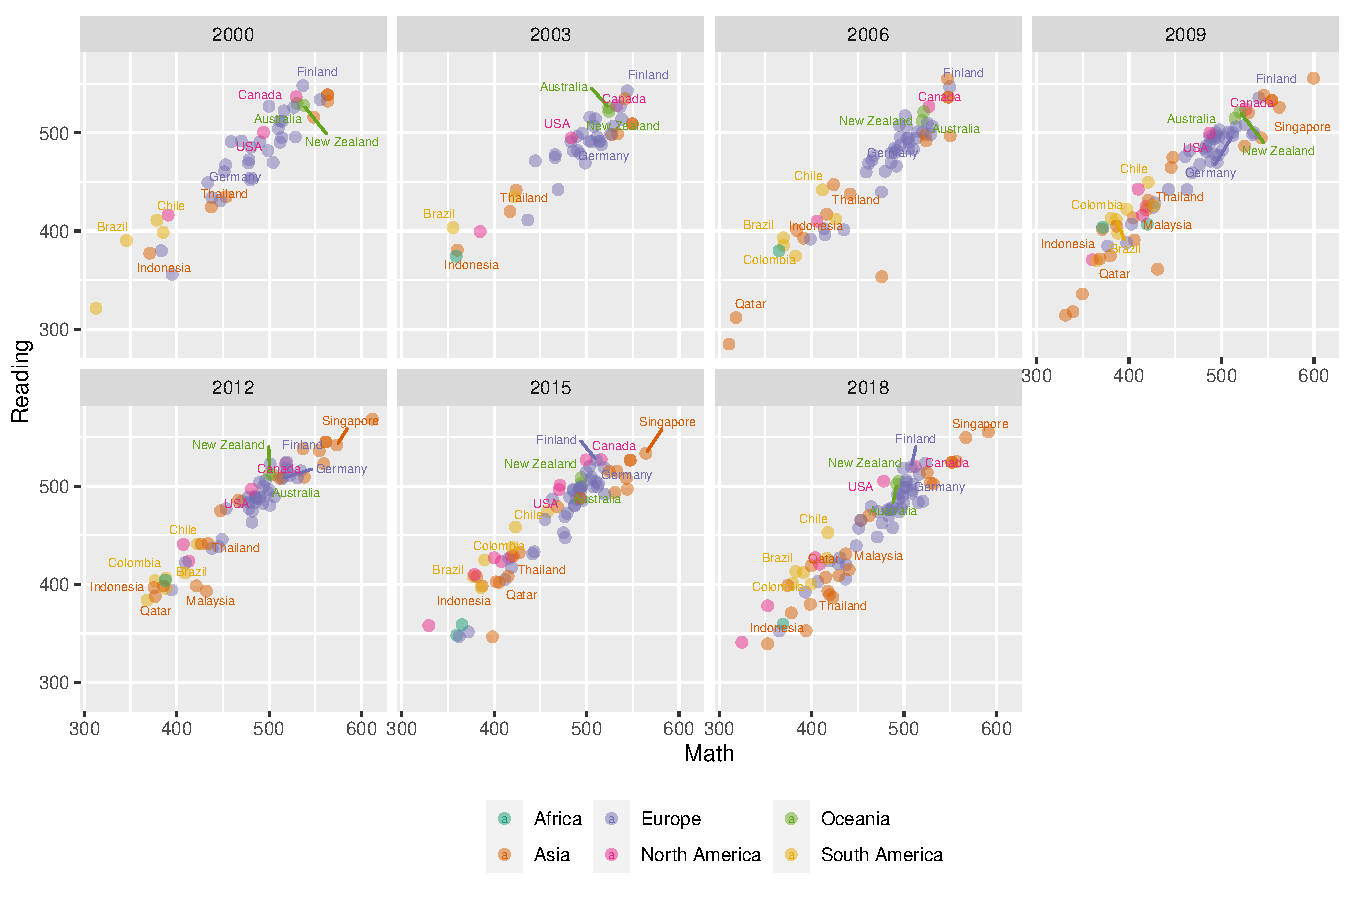
\includegraphics[width=1\linewidth]{learningtower_files/figure-latex/facet-time-1} \caption[Math and reading scores over time, with selected countries labelled]{Math and reading scores over time, with selected countries labelled. Colour indicates continent. Australia has quite stable scores over the years.}\label{fig:facet-time}
\end{figure}
\end{Schunk}

\hypertarget{discussion}{%
\section{Discussion}\label{discussion}}

Some things to say here

\bibliography{learningtower.bib}

\address{%
Priya Ravindra Dingorkar\\
Monash University\\%
Department of Econometrics and Business Statistics\\ Clayton,
Australia\\
%
\url{https://www.linkedin.com/in/priya-dingorkar/}\\%
%
\href{mailto:priyadingorkar@gmail.com}{\nolinkurl{priyadingorkar@gmail.com}}%
}

\address{%
Kevin Y.X. Wang\\
University of Sydney\\%
Data scientist\\ Illumina, Inc.\\ School of Mathematics and
Statistics\\ Sydney, Australia\\
%
\url{https://kevinwang09.github.io/}\\%
%
\href{mailto:kevinwangstats@gmail.com}{\nolinkurl{kevinwangstats@gmail.com}}%
}

\address{%
Dianne Cook\\
Monash University\\%
Department of Econometrics and Business Statistics\\ Clayton,
Australia\\
%
\url{http://dicook.org/}\\%
%
\href{mailto:dicook@monash.edu}{\nolinkurl{dicook@monash.edu}}%
}
